%%%%%%%%%%%%%%%%%%%%%%%%%%% asme2ej.tex %%%%%%%%%%%%%%%%%%%%%%%%%%%%%%%
% Template for producing ASME-format journal articles using LaTeX    %
% Written by   Harry H. Cheng, Professor and Director                %
%              Integration Engineering Laboratory                    %
%              Department of Mechanical and Aeronautical Engineering %
%              University of California                              %
%              Davis, CA 95616                                       %
%              Tel: (530) 752-5020 (office)                          %
%                   (530) 752-1028 (lab)                             %
%              Fax: (530) 752-4158                                   %
%              Email: hhcheng@ucdavis.edu                            %
%              WWW:   http://iel.ucdavis.edu/people/cheng.html       %
%              May 7, 1994                                           %
% Modified: February 16, 2001 by Harry H. Cheng                      %
% Modified: January  01, 2003 by Geoffrey R. Shiflett                %
% Use at your own risk, send complaints to /dev/null                 %
%%%%%%%%%%%%%%%%%%%%%%%%%%%%%%%%%%%%%%%%%%%%%%%%%%%%%%%%%%%%%%%%%%%%%%

%%% use twocolumn and 10pt options with the asme2ej format
\documentclass[twocolumn,10pt]{asme2ej}
%%\documentclass[twocolumn,15pt]


\usepackage{epsfig} %% for loading postscript figures
\usepackage{mathtools}   % loads »amsmath«
\usepackage{amssymb,amsmath}
\usepackage{amsfonts}
\usepackage{multirow}
%\usepackage{natbib}
\usepackage{relsize}
\usepackage{graphicx}
\usepackage{color}
\usepackage{comment}
%\usepackage{algorithm2e}


\newtheorem{theorem}{Theorem}[section]
\newtheorem{corollary}{Corollary}
\newtheorem*{main}{Main Theorem}
\newtheorem{lemma}[theorem]{Lemma}
\newtheorem{proposition}{Proposition}
\newtheorem{conjecture}{Conjecture}
\newtheorem*{problem}{Problem}
%\theoremstyle{definition}
\newtheorem{definition}[theorem]{Definition}
\newtheorem{remark}{Remark}
\newtheorem*{notation}{Notation}

\DeclarePairedDelimiter{\norm}{\lVert}{\rVert}

\newcommand{\II}{\mathbb{I}}
\newcommand{\overbar}[1]{\mkern 1.5mu\overline{\mkern-1.5mu#1\mkern-1.5mu}\mkern 1.5mu}
\newcommand{\ttt}{{\bf t}}





\title{New Definitions of Mean}

\author{Qianli Ma\thanks{Address all correspondence to this author.}\\ 
		\textbf{Gregory S. Chirikjian}
    \affiliation{
	Robot and Protein Kinematics Laboratory\\
	Laboratory for Computational Sensing and Robotics\\
	Department of Mechanical Engineering\\
	The Johns Hopkins University\\
	Baltimore, Maryland, 21218\\
    Email: \{mqianli1, gchirik1\}@jhu.edu
    }	
}


\begin{document}

\maketitle    

%%%%%%%%%%%%%%%%%%%%%%%%%%%%%%%%%%%%%%%%%%%%%%%%%%%%%%%%%%%%%%%%%%%%%%
\begin{abstract}
\it
Abstract to be added.
 
\end{abstract}

\section{Introduction}
We begin by defining a Gaussian probability distribution on $SE(3)$ (assuming the norm $\norm{\Sigma}$ is small) as
$$ \rho(H; M, \Sigma) = \frac{1}{(2\pi)^3 |\Sigma|^{\frac{1}{2	}}} e^{-\frac{1}{2}F(M^{-1}H)}$$
where $\norm{\Sigma}$ denotes the determinant of $\Sigma$ and
$$ F(H) = [\log^{\vee}(H)]^T \Sigma^{-1} [\log^{\vee}(H)].$$

Previously, in order to determine the mean of the convolution of two PDFs, Baker-Campbell-Hausdorff formula is used given the assumption that function $f_1$ and $f_2$ are both highly focused. If $X, Y \in se(3)$, 
\begin{equation} 
log(e^X e^Y) = X + Y + \dfrac{1}{2}[X,Y] + \dfrac{1}{12}\left([X, [X,Y]] + [Y,[Y,X]]\right) + ...
\label{BCH}
\end{equation}
If $X$ and $Y$ are further constrained to be small so that $\norm{X} \ll 1$ and $\norm{Y} \ll 1$, then the first order approximation of Eq.(\ref{BCH}) can be written as:
\begin{equation}
\log(e^X e^Y) = X + Y + \dfrac{1}{2}[X,Y]
\end{equation}
As shown in \cite{Wang08}, the mean of covariance of the convolution of two highly focused functions are: 
\begin{equation}
M_{1*2} = M_1 \, M_2 \,\,\, {\rm and} \,\,\, \Sigma_{1*2} = Ad(M_2^{-1}) \,\Sigma_{1}\, Ad^T(M_2^{-1}) + \Sigma_{2}
\label{meancovconvdef} \end{equation}
where
\begin{equation} 
Ad(H) = \left(\begin{array}{ccc}
R && \mathbb{O} \\
\widehat{{\bf x}} R && R \end{array}\right) 
\label{adjdef} \end{equation}




\section{Mean and Covariance of A Single Distribution on SE(3)}


\subsection{Order Approximation of $M$}
Though this approximation works well when the distribution of $X$ is treated as a Delta function, it fails to extend to the case where its distribution is a general PDF $f(X)$. In an alternative to the first order approximation using Baker-Campbell-Hausdorff formula, it is possible to only assume $M^{-1}H$ is small such that $\norm{M^{-1}H - \II} \ll 1$. Given the Taylor expansion of the matrix logarithm described as:
\begin{equation}
\log(\II + X) = X - \dfrac{1}{2}X^2 + \dfrac{1}{3}X^3 - ...
\end{equation}
Then it is straight forward to have:
\begin{equation}
\begin{split}
&\log(M^{-1}H) \\ 
= &\log(\II + (M^{-1}H - \II)) \\ 
= &\left(M^{-1}H - \II \right) - \left(M^{-1}H - \II \right)^2/2 + \left(M^{-1}H - \II \right)^3/3 - ...
\end{split}
\end{equation}
Given the definition of the mean $M$ of a probability density $f(H)$ as:
\begin{equation} 
\int_{SE(3)} \log(M^{-1} H) f(H) dH = \mathbb{O}  
\label{meandef} 
\end{equation}
The first order approximation of Eq.(\ref{meandef}) is:
\begin{equation}
\int_{SE(3)} (M^{-1}H - \II) f(H)dH \approx \mathbb{O}
\end{equation}

\begin{equation}
M^{-1}\int_{SE(3)} H f(H)dH \approx \II
\end{equation}
Define the first order approximation of $M$ as $\widehat{M}$:
\begin{equation}
\widehat{M} \doteq \int_{SE(3)}Hf(H)dH
\label{1st}
\end{equation}

 $$ f_A(H) = \frac{1}{n} \sum_{i=1}^{n} \delta(A_i^{-1} H) \,\,\, {\rm and} \,\,\, f_B(H) = \frac{1}{n} \sum_{i=1}^{n} \delta(B_i^{-1} H). $$
 If $f(H)$ is of the form of $f_A(H)$ given above, then
\begin{equation} \
\begin{split} &\sum_{i=1}^{n} \log(M_A^{-1} A_i) = \mathbb{O} {\rm \,\,\,\,\, and} \\
&\Sigma_A = \frac{1}{n} \sum_{i=1}^{n} \log^{\vee}(M_A^{-1} A_i) [\log^{\vee}(M_A^{-1} A_i)]^T.  
\label{datameancovconvdef} 
\end{split}
\end{equation}
Discrete version will be:
\begin{equation}
\widehat{M_{A}} \doteq \sum_{i=1}^{n} A_{i} \left( \frac{1}{n} \sum_{j=1}^{n}  \delta(A_j^{-1} A_{i})dH \right) = \dfrac{1}{n}\sum_{i=1}^{n}A_{i}
\label{1stmean}
\end{equation}
Note that $\widehat{M}$ is generally not a group element in $SE(3)$, and the corresponding $SE(3)$ version can be obtained by projecting $\widehat{M}$ into $SE(3)$ using singular value decomposition (SVD) technique.:
\begin{equation}
R_{\widehat{M}} = U \Sigma V^{T}
\label{proj}
\end{equation}
The rotation part of the projected $\widehat{M}$ (named as $\widehat{M}_{proj}$) is:
\begin{equation}
R_{\widehat{M}_{proj}} = VU^{T}
\label{1storth}
\end{equation}
When testing with no-noise data, $\hat{A}X - X\hat{B}$ is pretty good in rotation, while the error in translation is significant. This will be rectified in the 2nd order approximation as introduced in the next section.



\subsection{Second Order Approximation of $M$}
Take the second order approximation in Eq.(\ref{meandef}):
\begin{equation}
\int_{SE(3)} \left((M^{-1}H - \II) - \dfrac{1}{2}(M^{-1}H - \II)^2 \right)f(H)dH \approx \mathbb{O}
\label{2nd1}
\end{equation}
\begin{equation}
\int_{SE(3)} \left( 2M^{-1}H - \dfrac{1}{2}M^{-1}HM^{-1}H - \dfrac{3}{2} \II \right)f(H)dH \approx \mathbb{O}
\label{2nd2}
\end{equation}
Multiply $M$ on both side of Eq.(\ref{2nd2}):
\begin{equation}
\int_{SE(3)} \left( 2H - \dfrac{1}{2}HM^{-1}H -\dfrac{3}{2}M \right)f(H)dH \approx \mathbb{O}
\label{2nd3}
\end{equation}
Substituting Eq.(\ref{1st}) into Eq.(\ref{2nd3}), we have:
\begin{equation}
2\widehat{M} - \dfrac{1}{2}\int_{SE(3)}HM^{-1}Hf(H)dH - \dfrac{3}{2}M \approx \mathbb{O}
\end{equation}
The 2nd order approximation of $M$ is denoted by $\overbar{M}$ defined as:
\begin{equation}
2\widehat{M} - \dfrac{1}{2}\int_{SE(3)}H\overbar{M}^{-1}Hf(H)dH - \dfrac{3}{2}\overbar{M} = \mathbb{O}
\end{equation}

\begin{equation}
2\widehat{M} - \overbar{M}\dfrac{1}{2}\int_{SE(3)}\overbar{M}^{-1}H\overbar{M}^{-1}Hf(H)dH - \dfrac{3}{2}\overbar{M} = \mathbb{O}
\label{2ndm}
\end{equation}

\begin{equation}
2\widehat{M} - \dfrac{1}{2n}\sum_{i=1}^{n}A_{i}\overbar{M}^{-1}A_{i} - \dfrac{3}{2}\overbar{M} = \mathbb{O}
\label{2ndmean}
\end{equation}

\begin{equation}
\boxed{2\widehat{M} - \dfrac{1}{2}\widehat{M}\overbar{M}^{-1}\widehat{M} - \dfrac{3}{2}\overbar{M} = \mathbb{O}}
\end{equation}

Initial value of $\overbar{M}$ is important for the accuracy of its convergence. When $\overbar{M}_0 = \widehat{\widehat{M}}$, which means the initial guess of $\overbar{M}$ is obtained by another orthogonalization of $\widehat{M}$, the result is much better. 

Note: simulation shows that, given data streams without noise, if we minimize on the above cost function along all six directions of the Lie algebra, then the objective function is likely to fall into a local minimum that is not better than the 1st order approximation. Instead, we only minimize on the three translational directions defined by the corresponding Lie algebra and the result becomes better. The theoretical meaning behind this is still unknown. 

Currently, the length of search steps is adjusted dynamically to get object function out of local minimums that are not small enough. 

The second term of Eq.(\ref{2ndm}) is very similar to the definition of the covariance of $f(H)$, and maybe  $\overbar{M}$ can be updated using the information of the covariance. Also, take a look at the cubness of variance in the first volume. 
The same technique as in Eq.(\ref{proj}) can be employed to project $\widehat{M}$ into $SE(3)$.



\subsection{Numerical Experiments for Validation of the Second Order Approximation of the Mean of a PDF}


\begin{figure}[h]\label{mean_approx_rot}
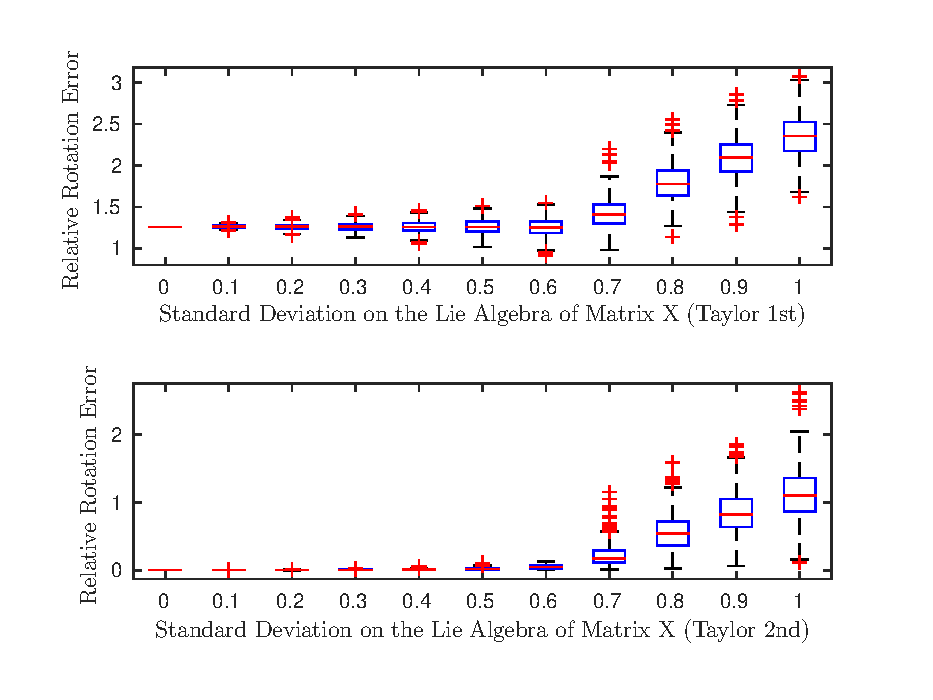
\includegraphics[scale = 0.60]{Mean_Definition_Figures/mean_rot_rel_10.eps}
\caption{Rotation Errors of 1st (up) and 2nd (down) Order Approximation With Respect to Different Noise Levels. Setup : (1) Number of Trials for Each Noise Level $n_t = 10$. (2) Number of Sample Points for Each Trial $n_s = 500$. }
\centering
\end{figure}

\begin{figure}[h]\label{mean_approx_tran}
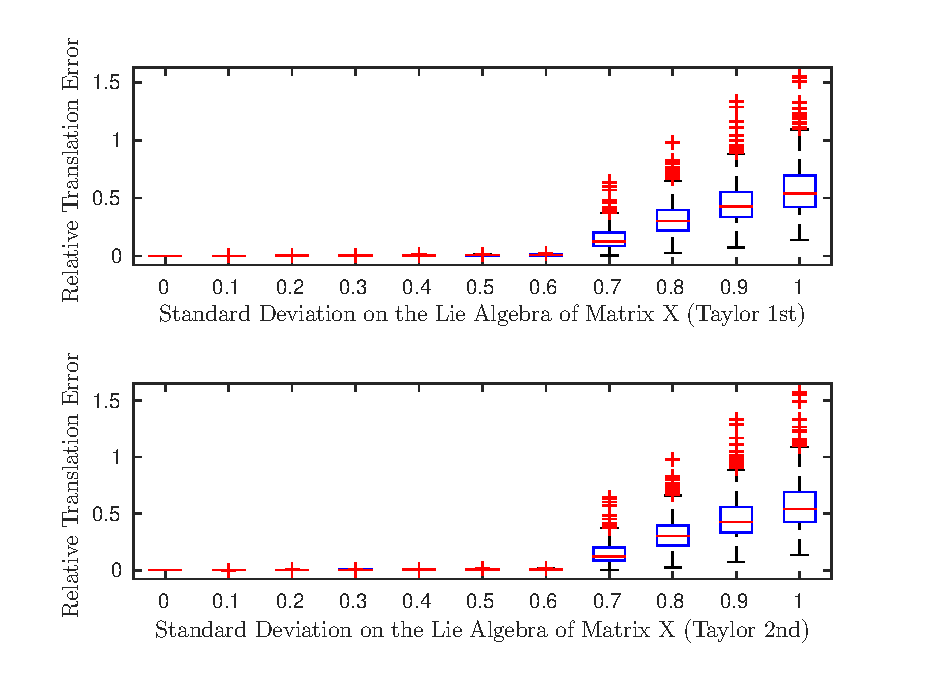
\includegraphics[scale = 0.60]{Mean_Definition_Figures/mean_trans_rel_10.eps}
\caption{Translation Errors of 1st (up) and 2nd (down) Order Approximation With Respect to Different Noise Levels. Setup : (1) Number of Trials for Each Noise Level $n_t = 10$. (2) Number of Sample Points for Each Trial $n_s = 500$. }
\centering
\end{figure}

\begin{figure}[h]\label{mean_approx_tran_close}
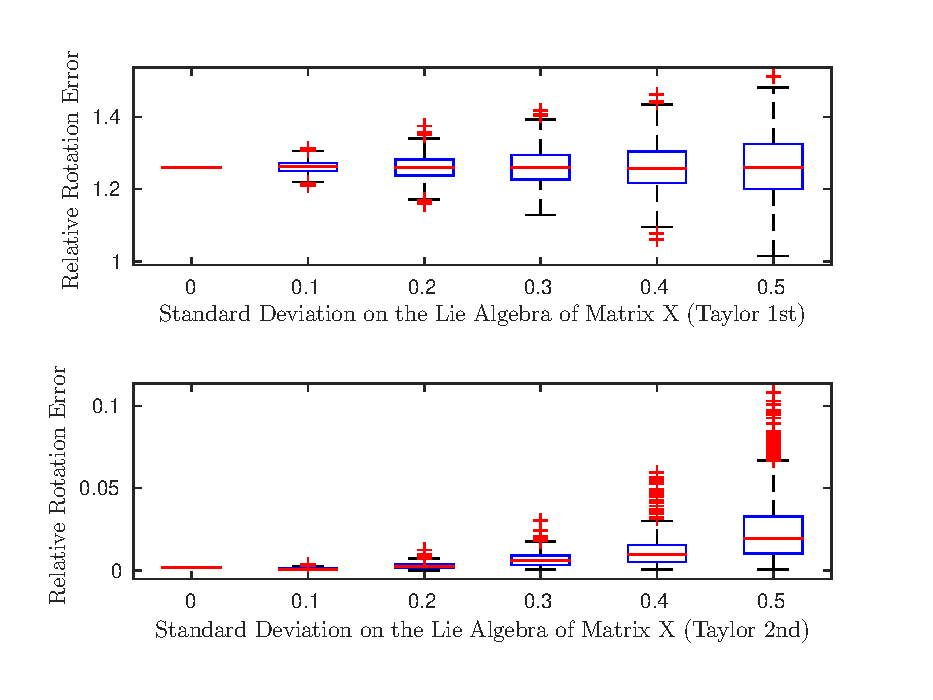
\includegraphics[scale = 0.60]{Mean_Definition_Figures/mean_rot_rel_5.eps}
\caption{A Closer Look at Fig.\ref{mean_approx_tran} with $\sigma = 0, 0.1, ... , 0.5$}
\centering
\end{figure}

\begin{figure}[h]\label{mean_approx_rot_close}
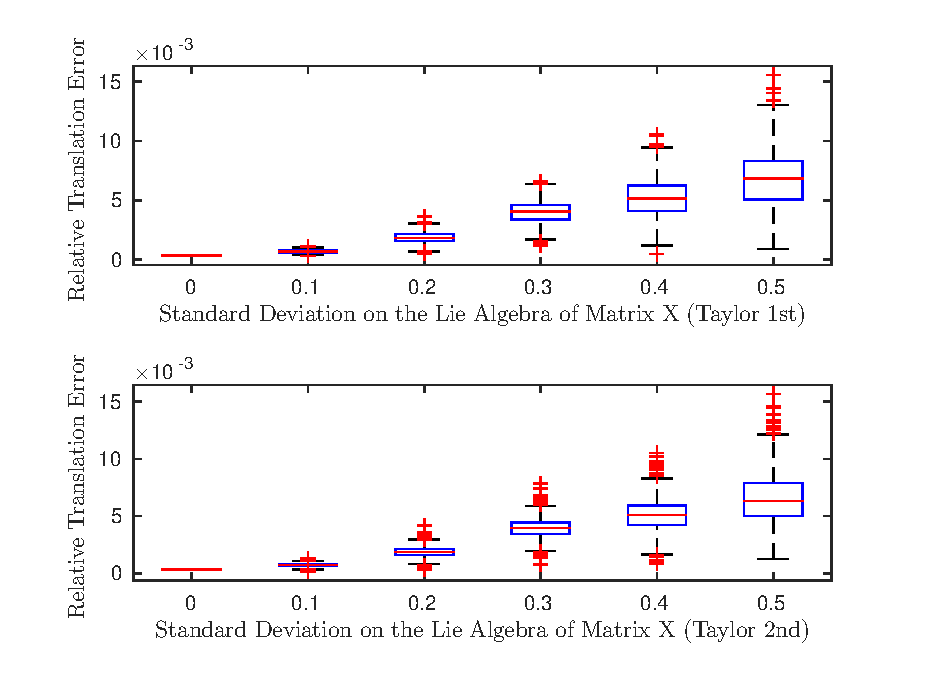
\includegraphics[scale = 0.60]{Mean_Definition_Figures/mean_trans_rel_5.eps}
\caption{A Closer Look at Fig.\ref{mean_approx_rot} with $\sigma = 0, 0.1, ... , 0.5$}
\centering
\end{figure}

Let $M_X$, $MX1$ and $MX2$ be the means of X obtained using Eq.(\ref{datameancovconvdef}), Eq.(\ref{1stmean} - \ref{1storth}) and Eq.(\ref{2ndmean}) respectively.  
\begin{figure}[h]
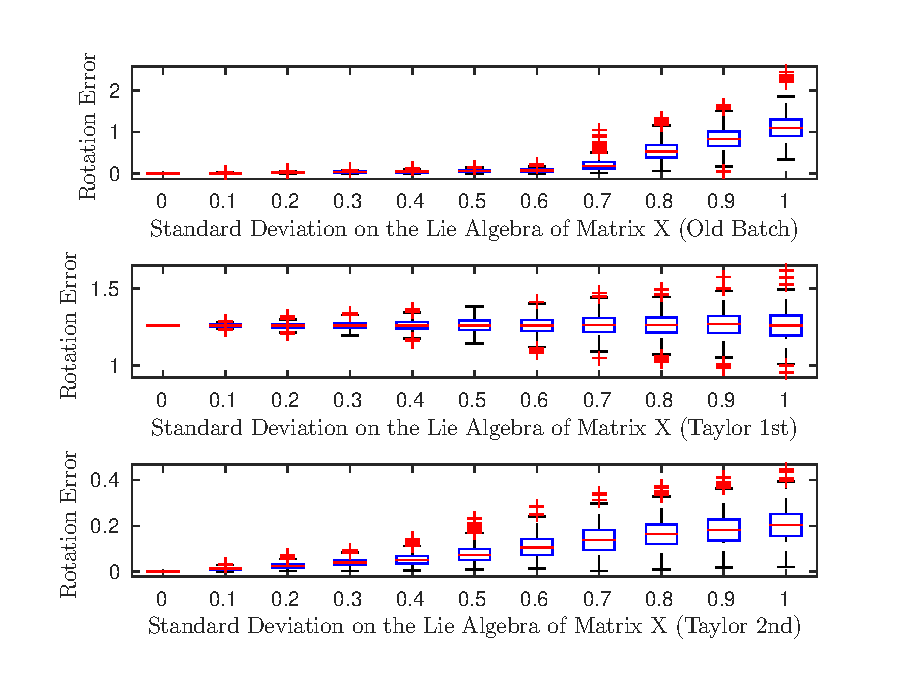
\includegraphics[scale = 0.60]{Mean_Definition_Figures/mean_rot_abs_10.eps}
\caption{Comparison of Rotation Errors With Respect to Different Noise Levels with Original Definition (up), 1st Taylor (mid) and 2nd Taylor (down). Setup : (1) Number of Trials for Each Noise Level $n_t = 10$. (2) Number of Sample Points for Each Trial $n_s = 500$. }
\centering
\label{mean_comp_tran}
\end{figure}

\begin{figure}[h]
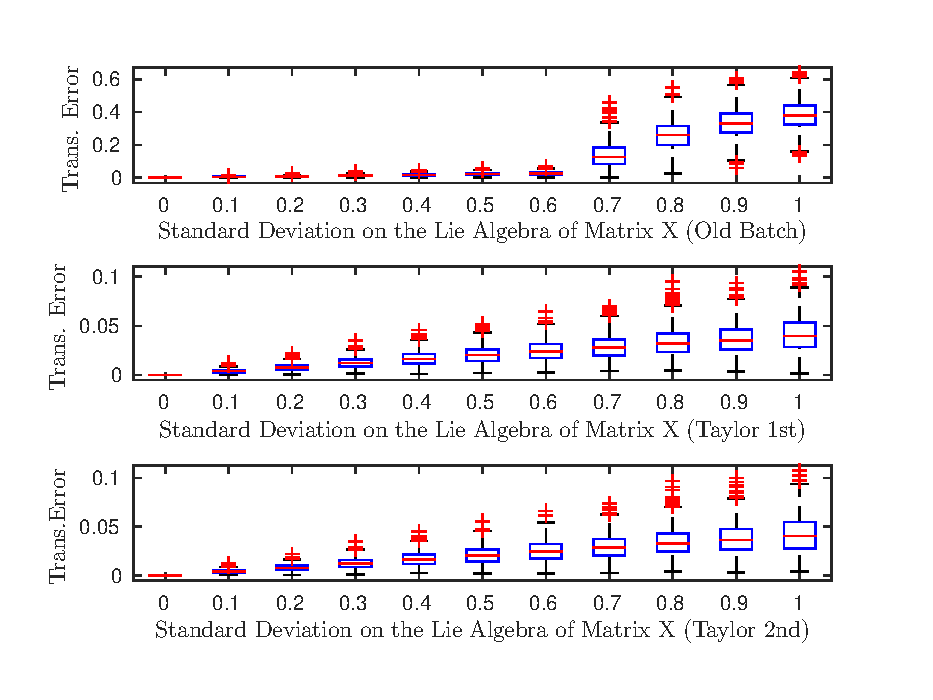
\includegraphics[scale = 0.60]{Mean_Definition_Figures/mean_trans_abs_10.eps}
\caption{Comparison of Translation Errors With Respect to Different Noise Levels with Original Definition (up), 1st Taylor (mid) and 2nd Taylor (down). Setup : (1) Number of Trials for Each Noise Level $n_t = 10$. (2) Number of Sample Points for Each Trial $n_s = 500$. }
\centering
\label{mean_comp_rot}
\end{figure}

\begin{figure}[h]
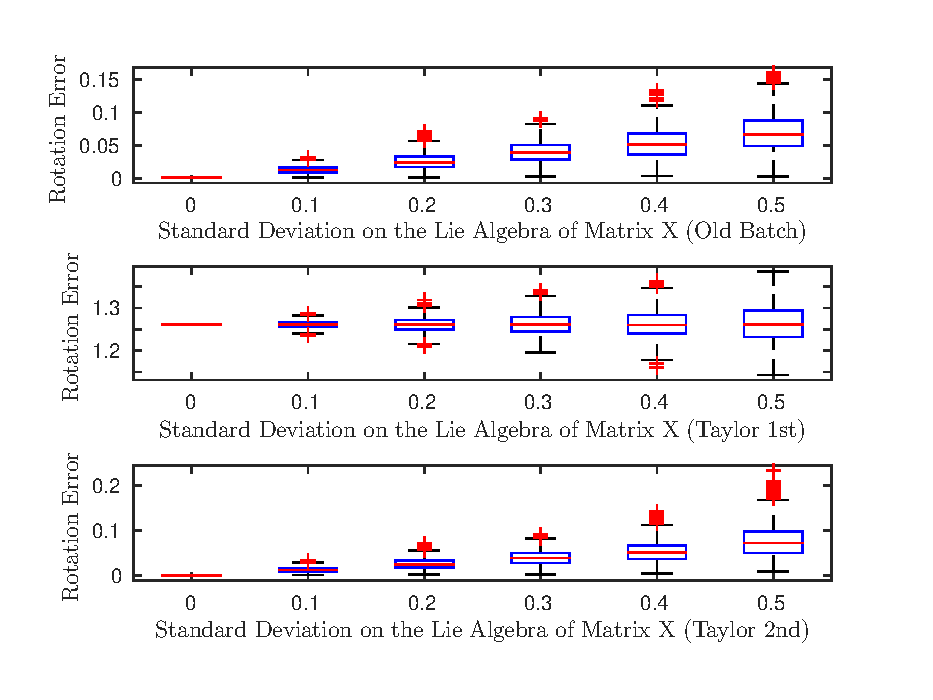
\includegraphics[scale = 0.60]{Mean_Definition_Figures/mean_rot_abs_5.eps}
\caption{A Close Look at Fig.\ref{mean_comp_tran} with $\sigma = 0, 0.1, ..., 0.5$ }
\centering
\end{figure}

\begin{figure}[h]
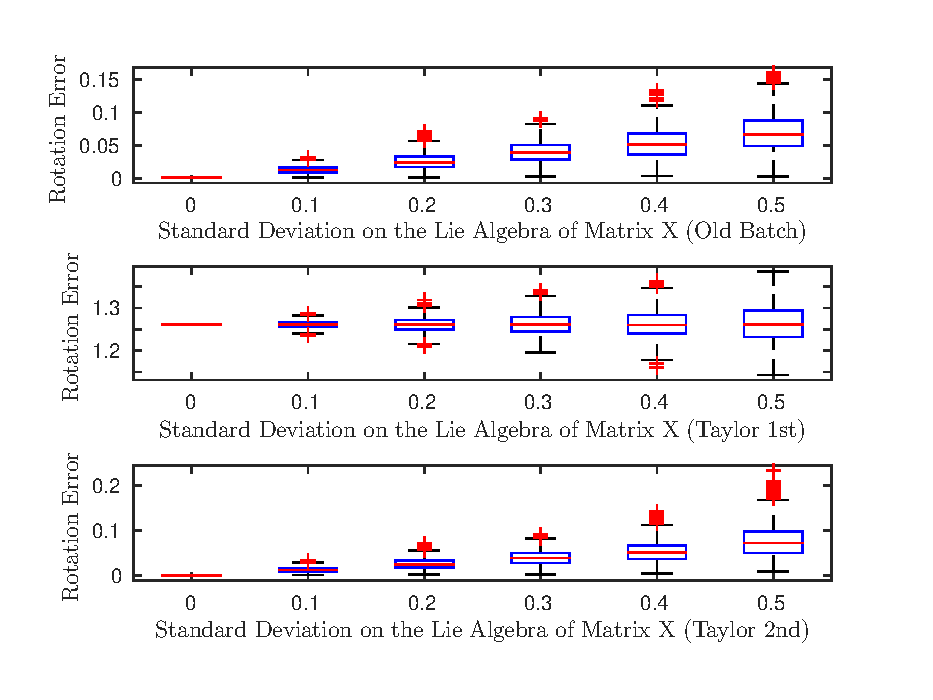
\includegraphics[scale = 0.60]{Mean_Definition_Figures/mean_rot_abs_5.eps}
\caption{A Closer Look at Fig.\ref{mean_comp_rot} with $\sigma = 0, 0.1, ..., 0.5$ }
\centering
\end{figure}

Number of iterations for each noise level is 10 and the number of sample points for each trial is 500. The following metrics are used for error comparison:
\begin{equation}
error_R = || R_X^{T} R_{X_{true}} ||_2
\end{equation}

\begin{equation}
error_t = \dfrac{||t_X - t_{X_{true}} ||_2 }{|| t_{X_{true}}||_2}
\end{equation}

Numerical simulation results are shown as in Fig.\ref{mean_approx_rot}, Fig.\ref{mean_approx_tran}, Fig.\ref{mean_approx_rot_close} and Fig.\ref{mean_approx_tran_close}.



\subsection{First Order Approximation of $\Sigma$}
Given the definition of the covariance $\Sigma$ of a PDF $f(H)$ as:
\begin{equation} 
\Sigma = \int_{SE(3)} \log^{\vee}(M^{-1} H) [\log^{\vee}(M^{-1} H)]^T  f(H) dH \label{meancovdef} \end{equation}
Its first order approximation $\widehat{\Sigma}$ can be written as:
\begin{equation}
\widehat{\Sigma} \doteq \int_{SE(3)} (M^{-1} H - \II)^{\vee} [(M^{-1} H - \II)^{\vee}]^T  f(H) dH
\label{1stCov}
\end{equation}
The discrete version for $\Sigma_{A}$ will be:
\begin{equation}
\Sigma_A = \frac{1}{n} \sum_{i=1}^{n} (M_A^{-1} A_i- \II)^{\vee} [(M_A^{-1} A_i- \II)^{\vee}]^T.  
\end{equation}
By defining $Q = M^{-1}H$, Eq.(\ref{1stCov}) can be written as:
\begin{equation}
\widehat{\Sigma} \doteq \int_{SE(3)} (Q - \II)^{\vee} [(Q - \II)^{\vee}]^T  f(Q) dQ
\end{equation}
A discrete version will be:
\begin{equation}
\Sigma = \frac{1}{n} \sum_{i=1}^{n} (Q_i - \mathbb{I})^{\vee} [(Q_i - \mathbb{I})^{\vee}]^T. 
\end{equation}
If $\norm{G - \II} \ll 1$, then $\Sigma = \widehat{\Sigma}$
\begin{equation}
(Q - \II)^{\vee} =
\left( 
\begin{matrix}
\dfrac{1}{2}(R -R^{T}) \\
\ttt
\end{matrix}
\right)
\end{equation}



\subsection{Second Order Approximation of $\Sigma$}
Let
\begin{equation}
P = (M^{-1} H - \II) - \dfrac{1}{2}(M^{-1}H - \II)^2
\end{equation}
Similarly, the second order approximation of $\Sigma$ is:
\begin{equation}
\bar{\Sigma} \doteq \int_{SE(3)} P^{\vee} [P^{\vee}]^T  f(H) dH
\label{2ndCov}
\end{equation}
which will be in a rather complex form. However, the calculation of the discrete version of this will be similar to how it is done in the 1st order approximation of the covariance.




\section{Mean and Covariance of the  Convolution between Two Distributions on $SE(3)$}
\subsection{First Order Approximation of $M_{1*2}$}
Given two functions, $f_1, f_2 \in (L^1 \cap L^2)(SE(3))$, the convolution is defined as:
\begin{equation}
(f_1 * f_2)(H) \doteq \int_{SE(3)} f_1(K) f_2(K^{-1} H) dK. 
\label{convdef}
\end{equation}
The corresponding mean $M_{1*2}$ will be given as:
\begin{equation}
\int_{SE(3)} \log(M_{1*2}^{-1}H) (f_1*f_2)(H)dH = \mathbb{O}
\end{equation}
If both $\Sigma_1$ and $\Sigma_2$ are very small, then $M_{1*2} \approx M_1 M_2$ as is used in the old Batch method. Without using this approximation, take the assumption that $M^{-1}H$ is small and we will have:
\begin{equation}
\int_{SE(3)}\int_{SE(3)} \left(M_{1*2}^{-1}H - \II \right)f_{1}(K)f_{2}(K^{-1}H)dKdH \approx \mathbb{O}
\end{equation}
Define $L = K^{-1}H$,
\begin{equation}
\int_{SE(3)}\int_{SE(3)} \left(M_{1*2}^{-1}KL - \II \right)f_{1}(K)f_{2}(L)dKdL \approx \mathbb{O}
\label{convTalor}
\end{equation}
(Note: when the integrating domain is the entire SE(3), this is Ok. However, when formulating the discrete version of the equation, this can be problematic because the integral domain is only a subset of SE(3) and $K^-1H$ can change the original integrating domain into a new one. The same problem can happen to Eq.(\ref{M12_2nd}).)

By using Eq.(\ref{1st}) twice, Eq.(\ref{convTalor}) becomes:
\begin{equation}
M_{1*2}^{-1} \widehat{M_1}\widehat{M_2} \approx \II
\end{equation}
It is straight forward to define $\widehat{M}_{1*2}$ as:
\begin{equation}
\boxed{\widehat{M}_{1*2} = \widehat{M_1}\widehat{M_2}}
\end{equation}
Note that though the definition of $\widehat{M}_{1*2}$ is similar to that in the old Batch method, no assumption on $\Sigma$ is made but $M^{-1}H$ is small. Moreover, in order to solve for the true $M_{1*2}$, projection of $\widehat{M}_{1*2}$ back onto $SE(3)$ is still required. 
There are two ways to solve for $M_{1*2}^{proj}$.
\begin{equation}
M_{1*2}^{proj}=
\begin{cases}
\left(\widehat{M_1}\widehat{M_2}\right)_{proj}\\
\widehat{M_{1}}_{proj}\widehat{M_{2}}_{proj}
\end{cases}
\label{b_old}
\end{equation}
The effectiveness of this approximation has been numerically simulated as shown in Fig.(\ref{rotXB}) and Fig.(\ref{tXB}).

%-----------------------------------------------%
%                                               %
%-----------------------------------------------%
\subsection{Second Order Approximation of $M_{1*2}$}
For simplicity, we drop the domain of integral $SE(3)$,
\begin{equation}
\int\int\left(2M_{1*2}^{-1}H - \dfrac{1}{2}M_{1*2}^{-1}HM_{1*2}^{-1}H - \dfrac{3}{2}\II \right)f_{1}(K)f_{2}(K^{-1}H)dKdH \approx \mathbb{O}
\end{equation}
Substitute $L = K^{-1}H$,
\begin{equation}
\int\int \left(2M_{1*2}^{-1}KL - \dfrac{1}{2}M_{1*2}^{-1}KLM_{1*2}^{-1}KL - \dfrac{3}{2}\II \right)f_{1}(K)f_{2}(L)dKdL \approx \mathbb{O}
\end{equation}
Employing the definition of $\widehat{M}$,
\begin{equation}
M_{1*2}^{-1}\widehat{M_{1}}\widehat{M_{2}} \approx \dfrac{1}{4} \int\int \left(M_{1*2}^{-1}KLM_{1*2}^{-1}KL \right)f_{1}(K)f_{2}(L)dKdL + \dfrac{3}{4}\II
\label{M12_2nd} 
\end{equation}
The discrete version of Eq.(\ref{M12_2nd}) is: 
\begin{equation}
\boxed{
\overbar{M}_{1*2}^{-1}\widehat{M_{1}}\widehat{M_{2}} = \dfrac{1}{4n^2} \sum_{i=1}^n \sum_{j=1}^n \overbar{M}_{1*2}^{-1}K_i L_j \overbar{M}_{1*2}^{-1}K_i L_j  + \dfrac{3}{4}\II
}
\label{2nd12}
\end{equation}
The effectiveness of this 2nd order approximation has been numerically simulated as shown in Fig.(\ref{rotXB}) and Fig.(\ref{tXB}). 

\begin{figure}[h]
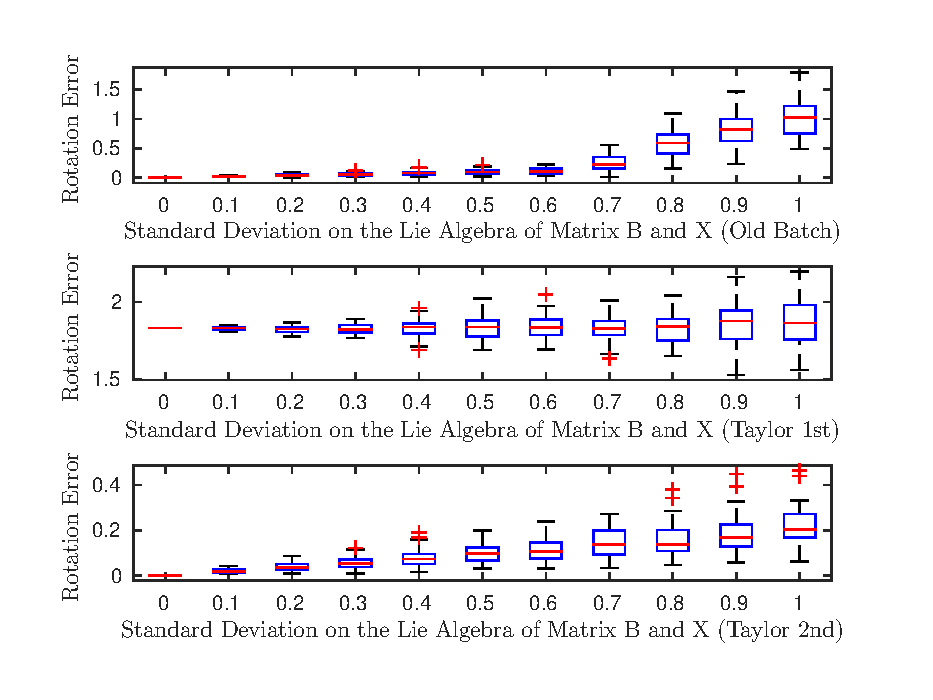
\includegraphics[scale=0.6]{col_mean_rot_error_1_10.eps}
\caption{Comparison of Translation Errors With Respect to Different Noise Levels Given One Pair of True X and True B}
\centering
\label{rotXB}
\end{figure}

\begin{figure}[h]
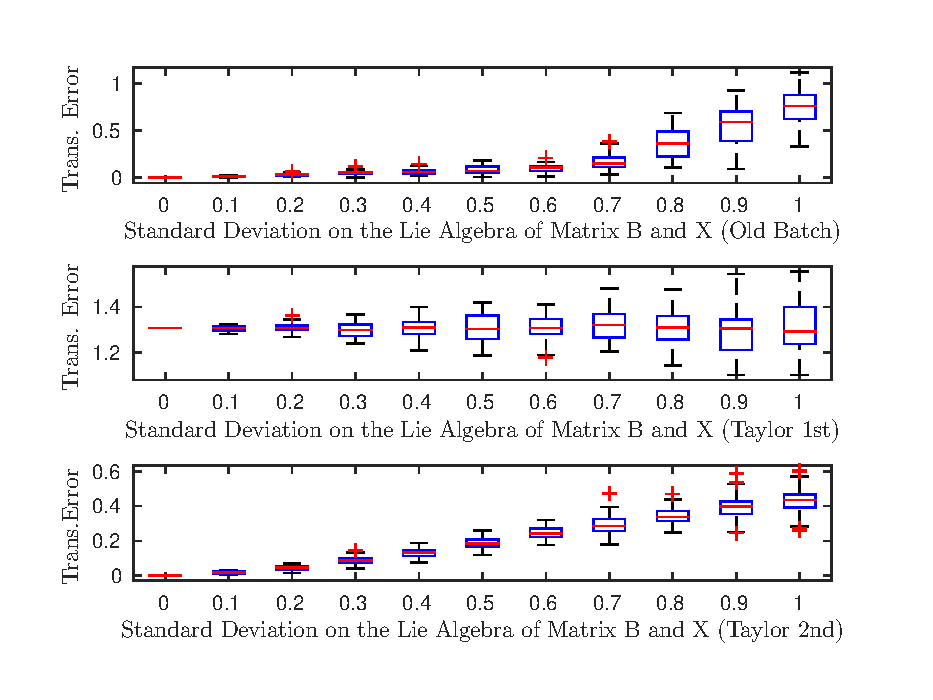
\includegraphics[scale=0.6]{col_mean_trans_error_1_10.eps}
\caption{Comparison of Translation Errors With Respect to Different Noise Levels Given One Pair of True X and True B}
\centering
\label{tXB}
\end{figure}

\begin{figure}[h]
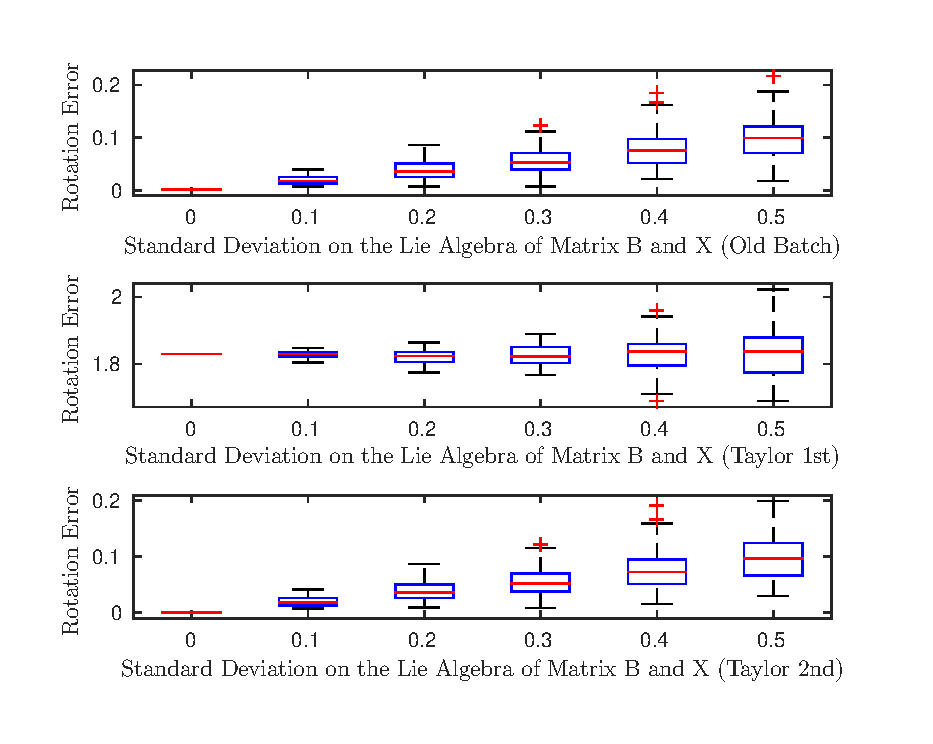
\includegraphics[scale=0.6]{col_mean_rot_error_1_6.eps}
\caption{Comparison of Translation Errors With Respect to Different Noise Levels Given One Pair of True X and True B}
\centering
\end{figure}

\begin{figure}[h]
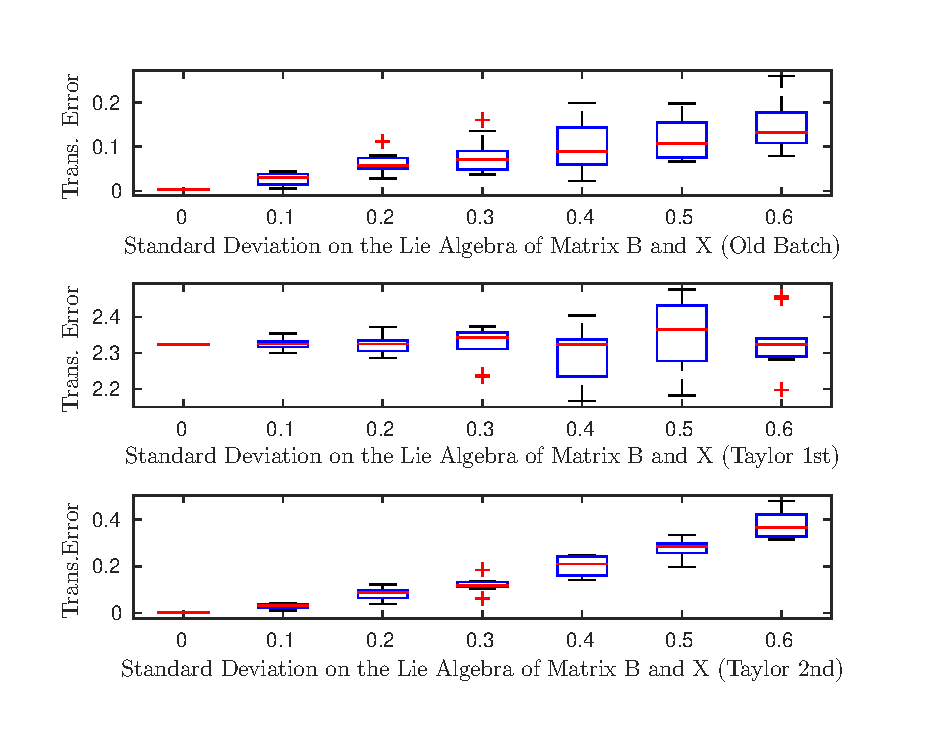
\includegraphics[scale=0.6]{col_mean_trans_error_1_6.eps}
\caption{Comparison of Translation Errors With Respect to Different Noise Levels Given One Pair of True X and True B}
\centering
\end{figure}

\subsection{1st and 2nd Taylor Approximations of the Convolution of Two Distributions on $SE(3)$}
\begin{figure}[h]\label{mean_conv_approx_rot}
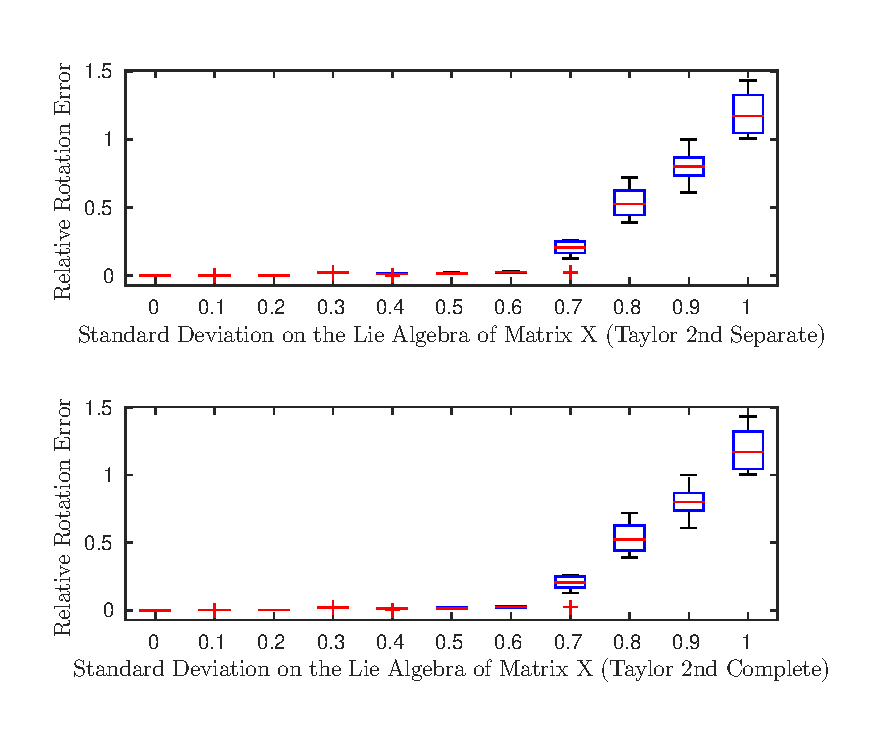
\includegraphics[scale = 0.60]{Mean_Definition_Figures/mean_conv_rot_rel_10.eps}
\caption{Rotation Errors of 1st (up) and 2nd (down) Order Approximation With Respect to Different Noise Levels. Setup : (1) Number of Trials for Each Noise Level $n_t = 10$. (2) Number of Sample Points for Each Trial $n_s = 200$. }
\centering
\end{figure}

\begin{figure}[h]\label{mean_conv_approx_tran}
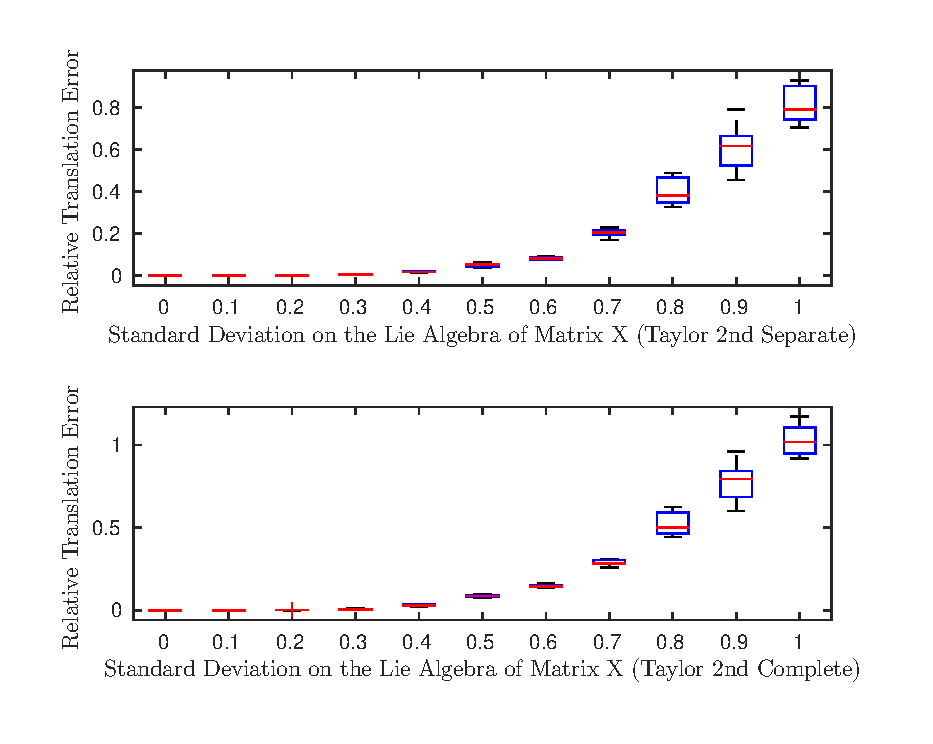
\includegraphics[scale = 0.60]{Mean_Definition_Figures/mean_conv_trans_rel_10.eps}
\caption{Translation Errors of 1st (up) and 2nd (down) Order Approximation With Respect to Different Noise Levels. Setup : (1) Number of Trials for Each Noise Level $n_t = 10$. (2) Number of Sample Points for Each Trial $n_s = 200$. }
\centering
\end{figure}

\begin{figure}[h]\label{mean_conv_approx_tran_close}
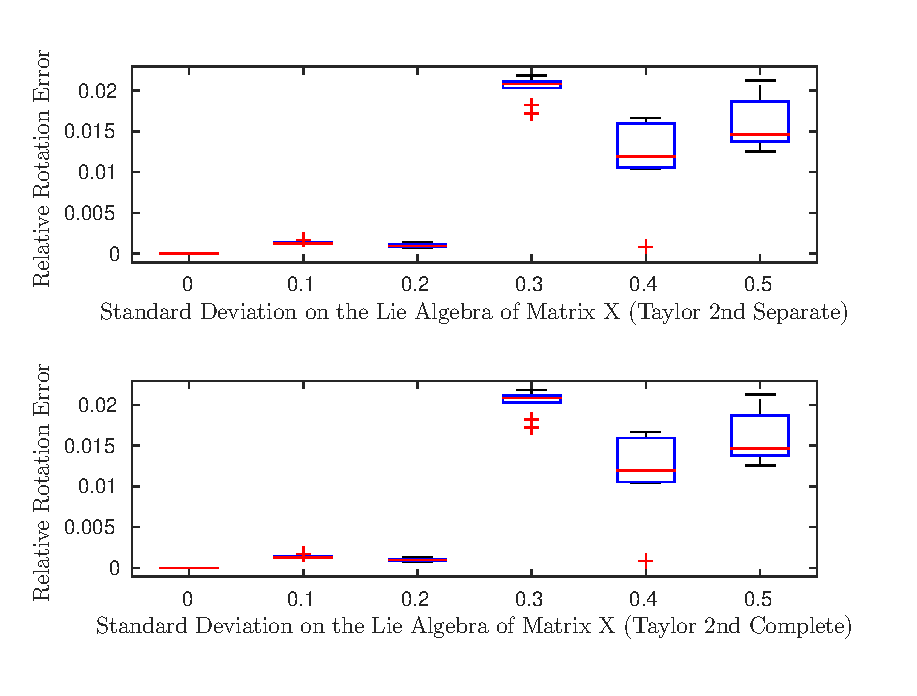
\includegraphics[scale = 0.60]{Mean_Definition_Figures/mean_conv_rot_rel_5.eps}
\caption{A Closer Look at Fig.\ref{mean_conv_approx_tran} with $\sigma = 0, 0.1, ... , 0.5$}
\centering
\end{figure}

\begin{figure}[h]\label{mean_conv_approx_rot_close}
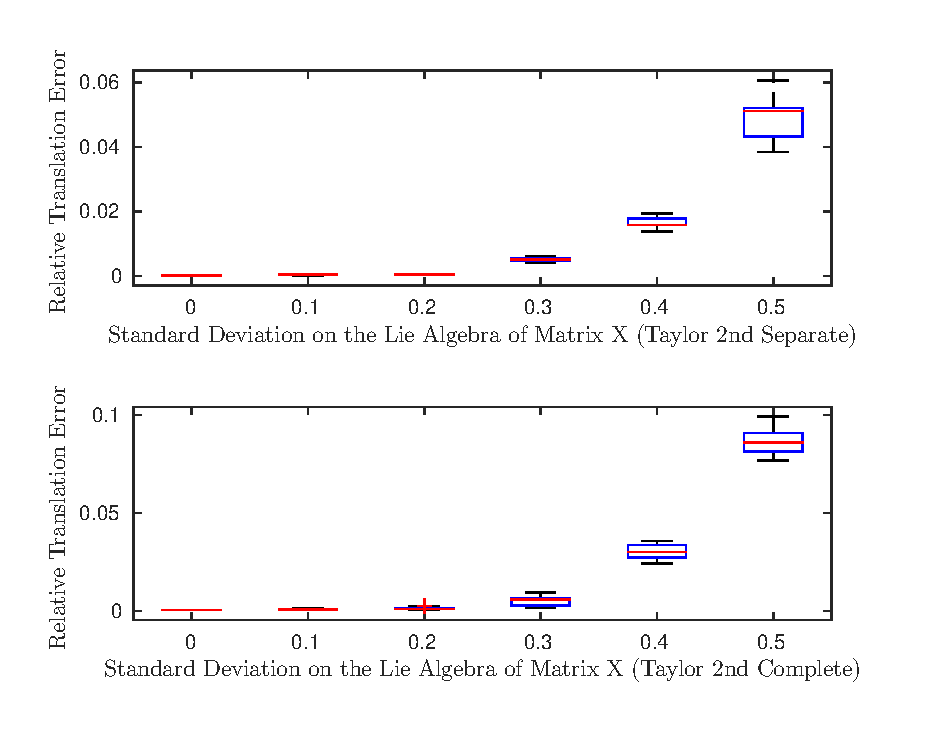
\includegraphics[scale = 0.60]{Mean_Definition_Figures/mean_conv_trans_rel_5.eps}
\caption{A Closer Look at Fig.\ref{mean_comv_approx_rot} with $\sigma = 0, 0.1, ... , 0.5$}
\centering
\end{figure}

\section{Error Comparison between AX and XB}
Given distributions on $A$, $X$, and $B$ originating from the equation $AX=XB$, the difference between $AX$ and $XB$ are numerically simulated by calculating the means of $f_A * f_X$, $f_X * f_B$ respectively, as shown in Fig.(\ref{rotaxxbconv}) and Fig.(\ref{taxxbconv}). 
\begin{figure}[h]
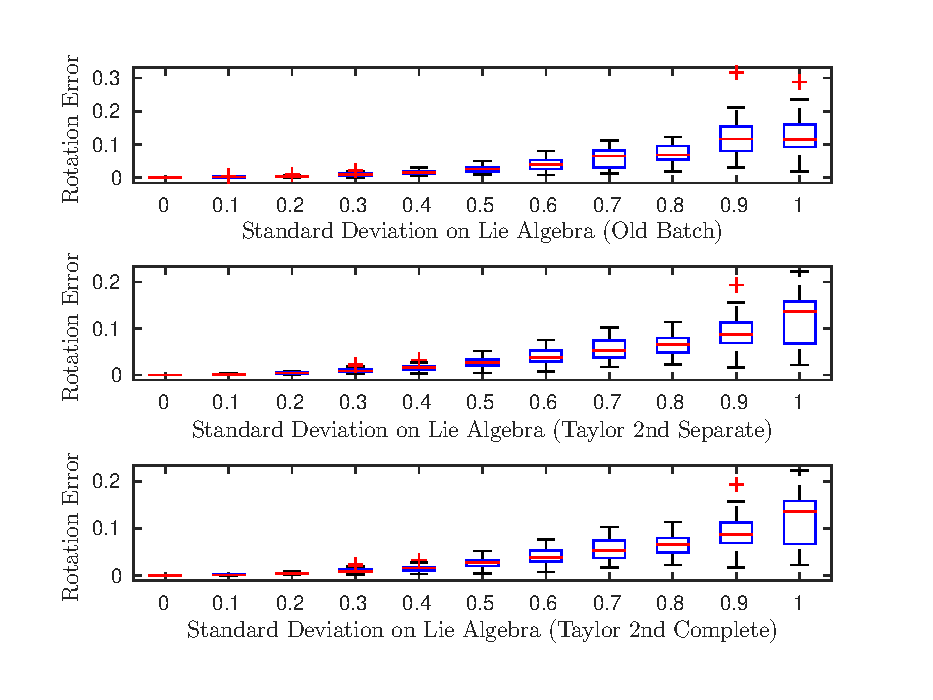
\includegraphics[scale=0.6]{ax_xb_mean_rot_error_1_10.eps}
\caption{AX and XB Error Comparison of Translation With Respect to Different Noise Levels}
\centering
\label{rotaxxbconv}
\end{figure}

\begin{figure}[h]
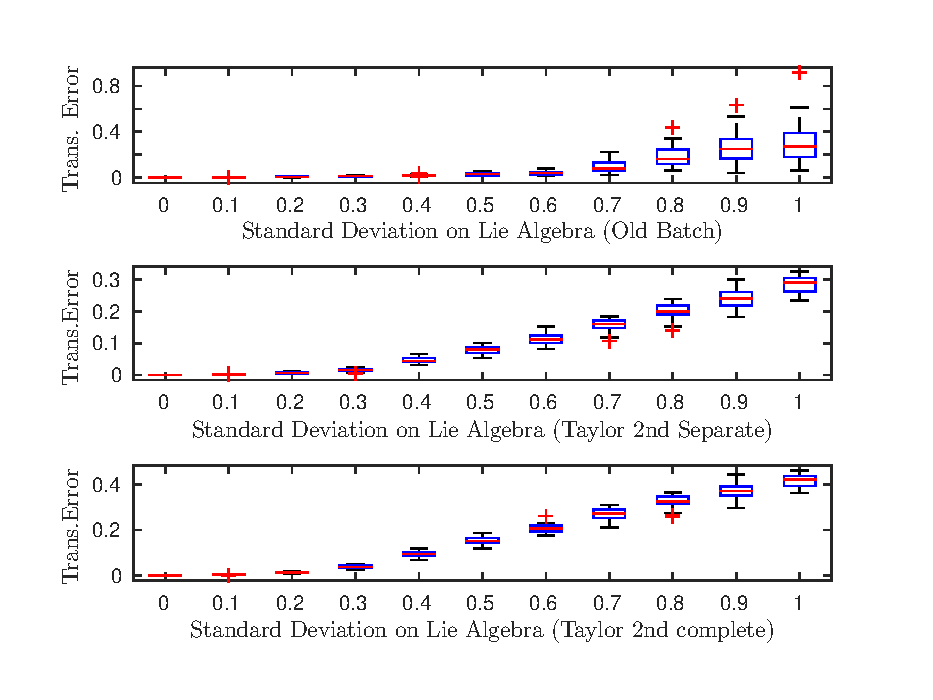
\includegraphics[scale=0.6]{ax_xb_mean_trans_error_1_10.eps}
\caption{AX and XB Error Comparison of Translation With Respect to Different Noise Levels}
\centering
\label{taxxbconv}
\end{figure}

\begin{figure}[h]
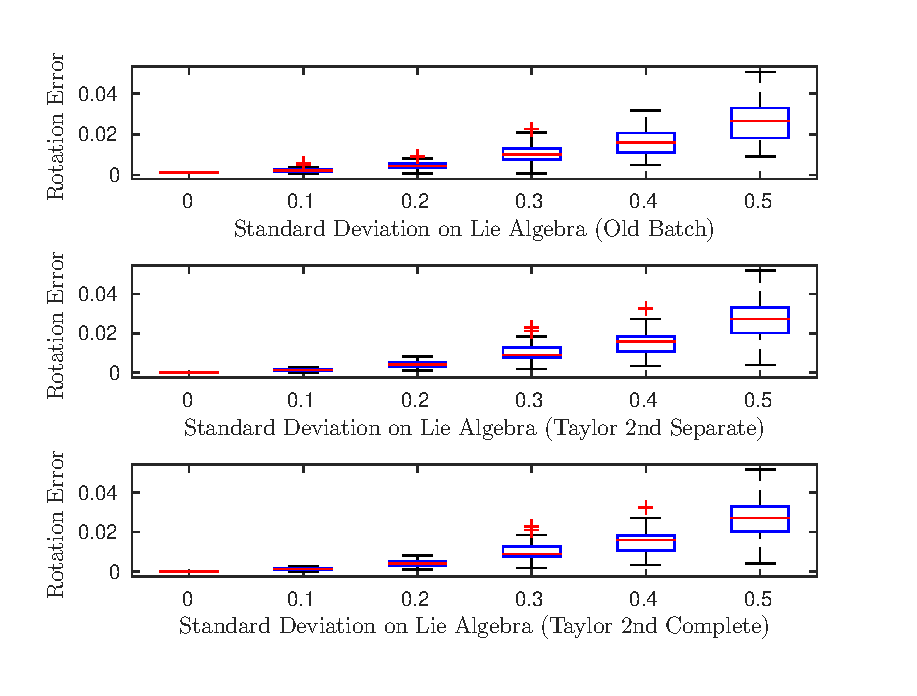
\includegraphics[scale=0.6]{ax_xb_mean_rot_error_1_6.eps}
\caption{AX and XB Error Comparison of Translation With Respect to Different Noise Levels}
\centering
\end{figure}

\begin{figure}[h]
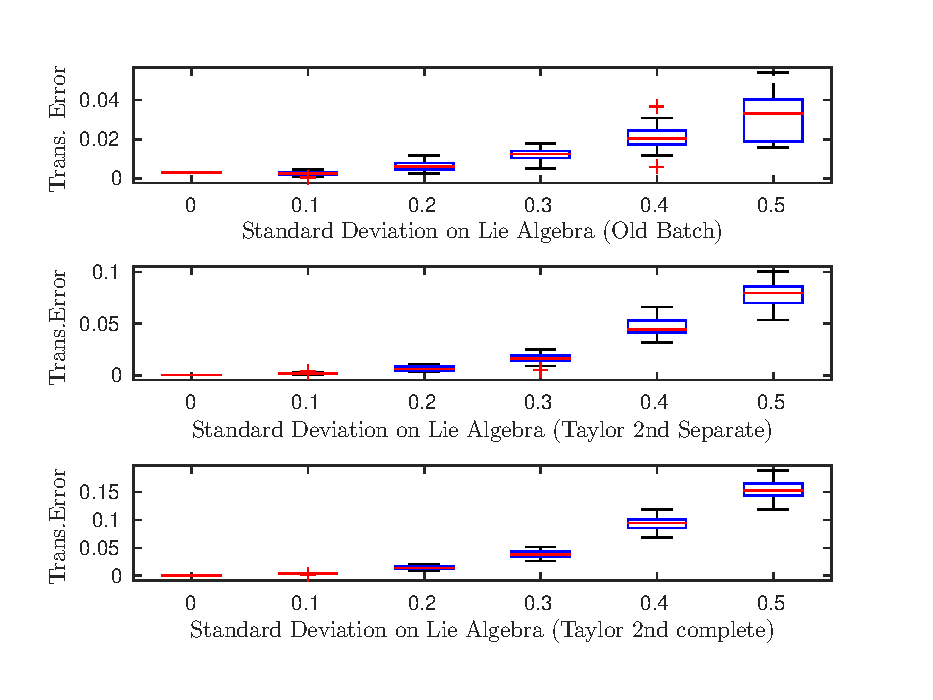
\includegraphics[scale=0.6]{ax_xb_mean_trans_error_1_6.eps}
\caption{AX and XB Error Comparison of Translation With Respect to Different Noise Levels}
\centering
\end{figure}

\section{Convolution of $XBX^{-1}$}
Treating $X$ as a probability distribution, then the following equation holds only when $A$ and $B$ have the same noise level (or similar distribution):
\begin{equation}
(f_A*f_X)(g) = (f_X*f_B)(g)
\end{equation}
However, in the real world, the noise levels on $A$ and $B$ are different, and different forms of convolution should be chosen accordingly. For example, when the noise level on $A$ is larger, the following equation can be used:
\begin{equation}
f_A(g) = \left(f_X*f_B*f_{X^{-1}}\right)(g)
\label{conv}
\end{equation}
The goal becomes to compare $M_A$ and $M_{X*B*X^{-1}}$ by using Eq.(\ref{2nd12}) twice. The first stage is just to verify the effectiveness of Eq.(\ref{conv}) given known data sets of $A$, $B$ and $X$.
\begin{equation}
\boxed{
\overbar{M}_{X*B}^{-1}\widehat{M_{X}}\widehat{M_{B}} = \dfrac{1}{4n^2} \sum_{i=1}^n \sum_{j=1}^n \overbar{M}_{X*B}^{-1}X_i B_j \overbar{M}_{X*B}^{-1}X_i B_j  + \dfrac{3}{4}\II}
\label{2ndXB}
\end{equation}

\begin{equation}
\overbar{M}_{X*B*X^{-1}}^{-1}\widehat{M}_{X*B}\widehat{M}_{X^{-1}} = \dfrac{1}{4n^2} \sum_{j=1}^n \overbar{M}_{X*B*X^{-1}}^{-1} \overbar{M}_{X*B} X_j^{-1} \overbar{M}_{X*B*X^{-1}}^{-1} \overbar{M}_{X*B} X_j^{-1}  + \dfrac{3}{4}\II
\label{2ndXBX}
\end{equation}

An alternative form is:
\begin{equation}
\begin{split}
& \boxed{\overbar{M}_{X*B*X^{-1}}^{-1}\widehat{M}_{X}\widehat{M}_{B}
\widehat{M}_{X^{-1}}} \\ 
& \boxed{= \dfrac{1}{4n^2} \sum_{i=1}^n \sum_{j=1}^n \sum_{k=1}^n  \overbar{M}_{X*B*X^{-1}}^{-1} X_{i} B_{j} X_k^{-1} \overbar{M}_{X*B*X^{-1}}^{-1} X_{i} B_{j} X_k^{-1}  + \dfrac{3}{4}\II}
\end{split}
\end{equation}

Error Metric 1:
\begin{equation}
error_R = ||\text{log}(R_{M_{A*X}}^{T} R_{M_{X*B}})||_2
\end{equation}

\begin{equation}
error_t = \dfrac{||t_{M_{A*X}} - t_{M_{X*B}}||_2}{||t_{M_{X*B}}||}
\end{equation}

Error Metric 2:
\begin{equation}
error_R = ||\text{log}(R_{M_{A}}^{T} R_{M_{X*B*X^{-1}}})||_2
\end{equation}

\begin{equation}
error_t = \dfrac{||t_{M_A} - t_{M_{X*B*X^{-1}}}||_2}{||t_{M_{X*B*X^{-1}}}||}
\end{equation}
where $M_{X*B*X^{-1}} = M_X M_B M_X^{-1}$ according to the old Batch method.

\begin{figure}[h]
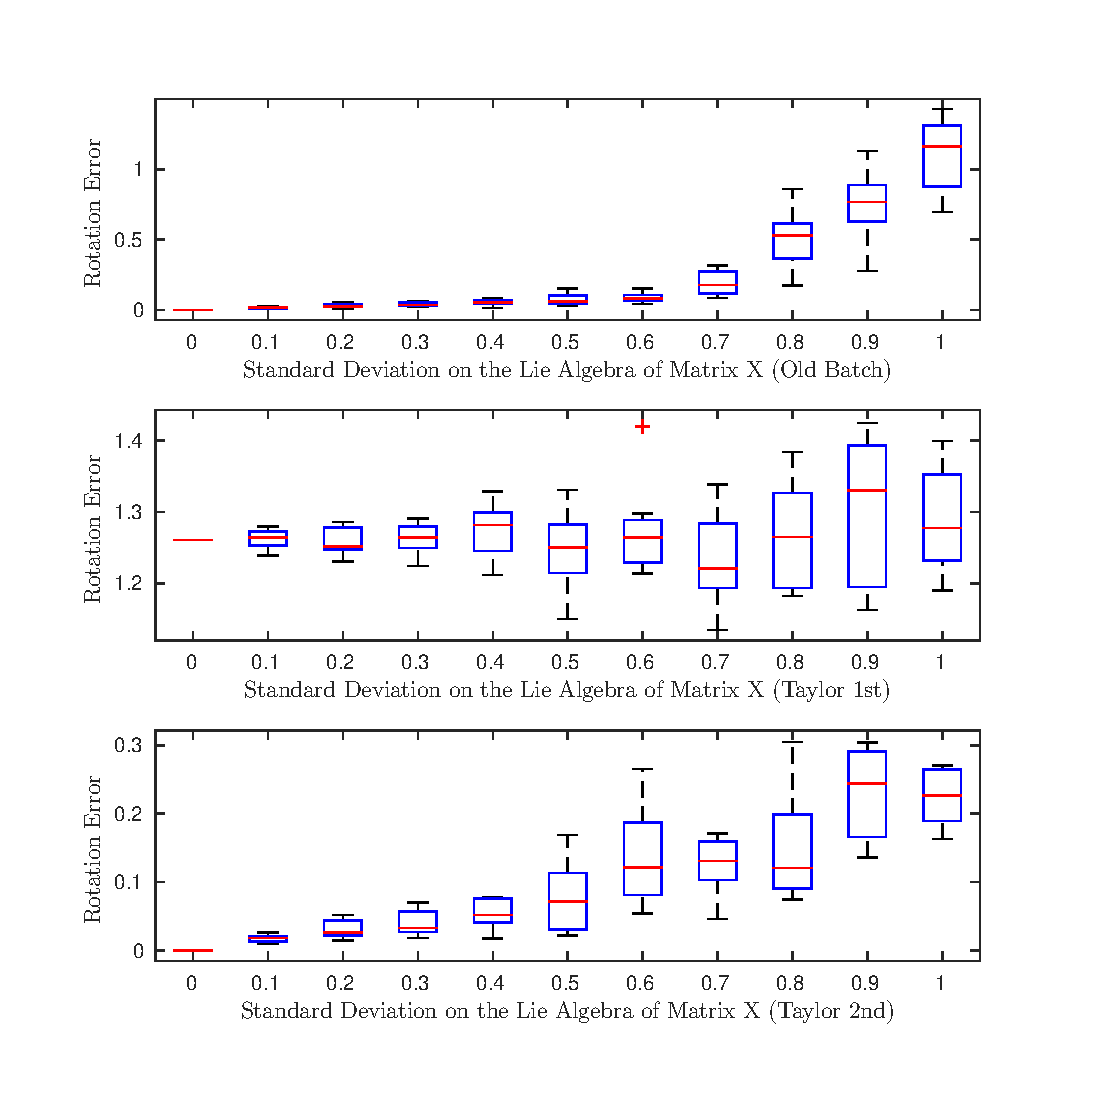
\includegraphics[scale=0.5]{mean_rot_error.eps}
\caption{$A$ and $XBX^{-1}$ Error Comparison of Translation With Respect to Different Noise Levels}
\centering
\label{rotaxbxconv}
\end{figure}

\begin{figure}[h]
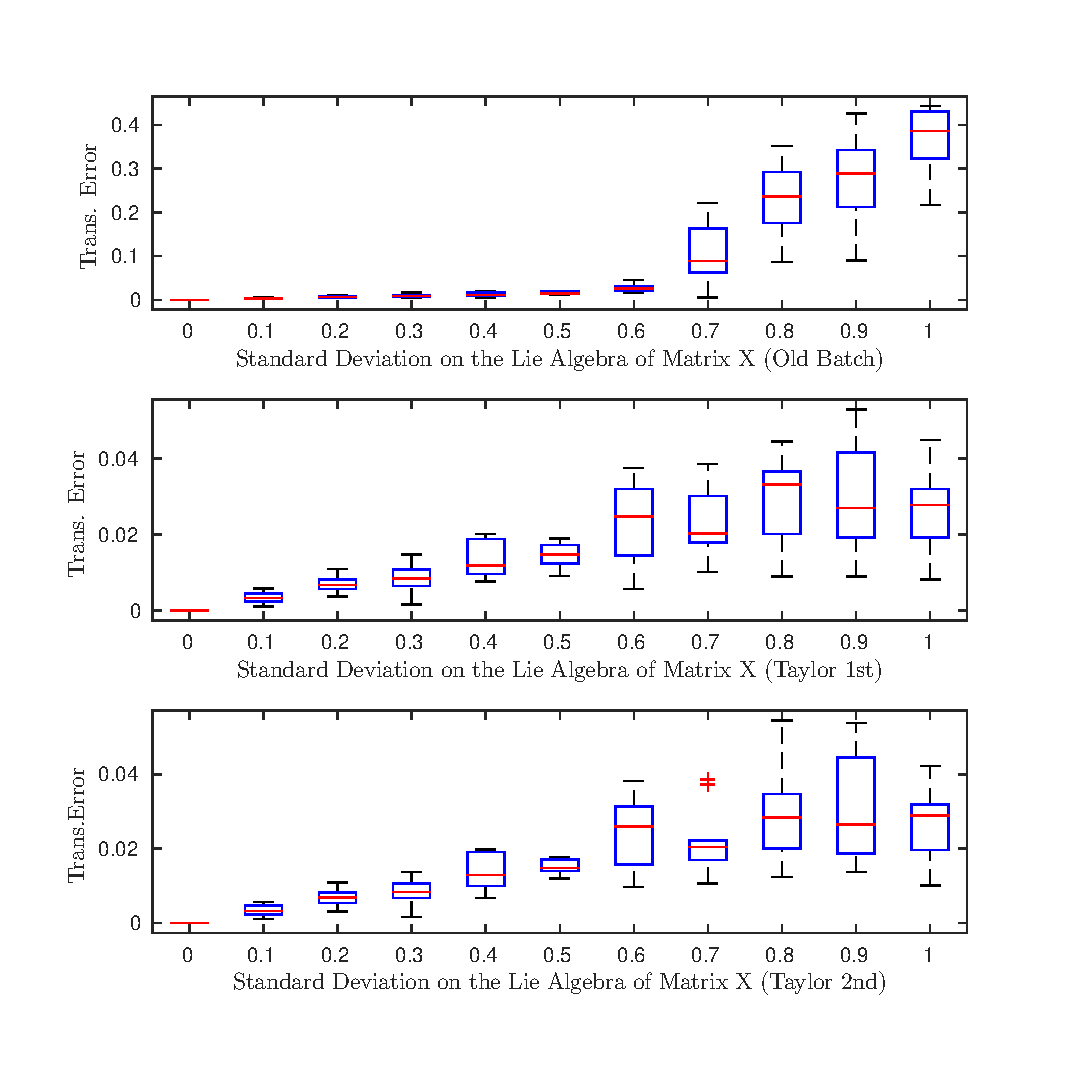
\includegraphics[scale=0.5]{mean_trans_error.eps}
\caption{$A$ and $XBX^{-1}$ Error Comparison of Translation With Respect to Different Noise Levels}
\centering
\label{taxbxconv}
\end{figure}

\section{Problem}
How to fit the information of covariance is still unknown, but the definition of the mean itself contains some information that is related to its covariance which might or might not have had a positive impact on the computation of the mean. 

How to solve for $X$ given $\{A\}$ and $\{B\}$ is still unclear. An initial guess of $X$ might be needed for Eq.(\ref{2nd12}) to calculate $M_{1*2}$ and as well as $M_{2*3}$. Then $M_{A*X} = M_{X*B}$ or $M_{A} = M_{X*B*X^{-1}}$ is treated as an object function to optimize on $X$ which is $M_2$ here. Moreover, though only 1st order approximations of $A$, $B$ and $X$ showed up in Eq.(\ref{2nd12}), it might be still possible to replace $A$ and $B$ with their 2nd order approximations to achieve a better $X$

\section{Fourier Transform on Functions of SE(3)}
Note: this is possible future work and will mostly likely be a separate paper.

For PDF version of $AX=XB$ as:
\begin{equation}
\rho_{A}(g) = \left( \rho_{X} * \rho_{B} * \rho_{X^{-1}} \right)(g)
\end{equation}
The equivalent form under Fourier transformation on both sides is:
\begin{equation}
\widehat{\rho}_{A}(g) = \left(\widehat{\rho}_{X}*\widehat{\rho}_{B}*\widehat{\rho}_{{X}^{-1}}\right)(g)
\end{equation}
The above equation can be used given any clouds of $A$ and $B$ without the assumption of highly focused distribution. 

Define a Gaussian by defining a diffusion equation and tuning its parameters. (Read Chapter 12 and 20 of the blue book. Tim Barfort Covariance Propagation. Corrected version of Wang's paper.)








% Here's where you specify the bibliography style file.
% The full file name for the bibliography style file 
% used for an ASME paper is asmems4.bst.
\bibliographystyle{asmems4}

% Here's where you specify the bibliography database file.
% The full file name of the bibliography database for this
% article is asme2e.bib. The name for your database is up
% to you.
\bibliography{New_Batch}
\end{document}